Introduzione alla sezione

\subsection{Studio della catena cinematica}
\label{ssez:cat_cine}

Consistono in 16 movimenti di sollevamento
di cui i primi 8 sono considerati corretti,
gli altri errati.
I sollevamenti sono effettuati a gomito vincolato,
quindi soltanto con l'avambraccio.
Durante i movimenti ``giusti'' la traiettoria \`e mantenuta
il pi\`u possibile dritta, mentre durante quelli ``sbagliati''
si devia dall'asse verticale.

Il cellulare \`e tenuto in mano in maniera
che lo schermo guardi nella stessa direzione del palmo.
Il polso \`e rigido.

\begin{figure}
  \centering
	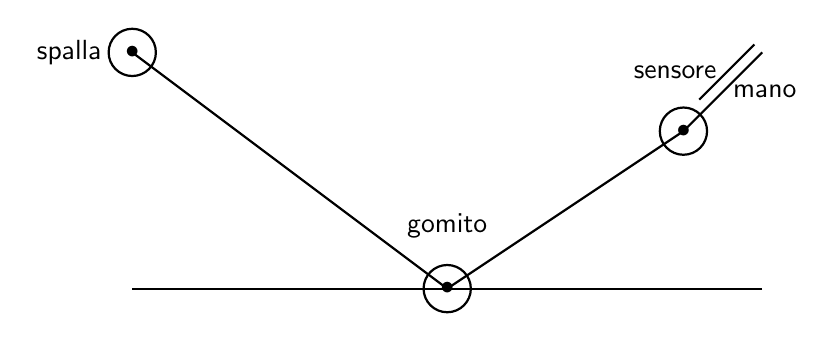
\begin{tikzpicture}[%
molla/.style={decorate,decoration={snake,post length=5,amplitude=5,pre length=5,segment length=5}, thick},
thick%
]
\sffamily \sansmath
%	\draw [help lines] (0, 0) grid (8, 5);
	
	\draw (8, 0) -- (0, 0);
	
	\draw (0, 3) circle (0.3)
		node at (0, 3) {$\bullet$};
	\node [] at (-.8, 3) {spalla};
	\draw (0, 3) -- (4, 0);
	\draw (4, 0) circle (0.3)
		node {$\bullet$};
	\node [] at (4, 0.8) {gomito};
	\draw (4, 0) -- (7, 2);
	\draw (7, 2) circle (0.3)
		node {$\bullet$};
	\draw (7, 2) -- (8, 3)
		node [pos=0.5, right] {mano};
	\draw (7.2, 2.4) -- (7.9, 3.1)
		node [pos=0.5, left] {sensore};

  \end{tikzpicture}
  \caption{Schema approssimativo.}
  \label{fig:gomito2}
\end{figure}

\subsection{Specifiche tecniche}
Forse a questo punto non sono granch\'e interessanti.

\subsection{Il punto di vista biomeccanico}
Fissata che sia la posizione della punta del gomito,
l'avambraccio ha tre gradi di libert\`a di rotazione.
Il polso pu\`o ruotare in altri due modi,
per un totale di cinque gradi di libert\`a.

In questa dimostrazione si cerca di sopprimere
i movimenti del polso e la rotazione sull'asse dell'avambraccio.
Fatto questo, si considera corretta l'esecuzione del movimento
quando non c'\`e variazione dell'angolo longitudinale
ma solo di quello latitudinale (vedi \textsc{Figura \ref{fig:gomito1}}).

Utilizzando i formalismi della robotica
%\footnote{ \cite{deluca}}
si pu\`o scrivere la \textsc{Tabella \ref{tab:robo}}.
Il sistema di riferimento $S_{3}$ \`e quello del telefonino.
In realt\`a sarebbe pi\`u corretto scrivere il sistema $S_{0}$
con l'asse $z$ verso l'alto e l'asse $y$ entrante foglio
(pi\`u una questione di convenzioni che di comodit\`a),
oppure con parallelo a $S_{3}$ in posizione di riposo
(con $x$ uscente dal foglio).

Secondo questa notazione:
\begin{itemize}
	\item [$\theta_{1}$] {$\in [0, \pi/2]$ \`e l'unico parametro che si vuole variare}
	\item [$\theta_{2}$] {$\in [-\pi/2, \pi/2]$ dovrebbe rimanere fisso, meglio se nullo}
	\item [$\alpha_{1}$] la rotazione attorno a $y_{1}$ \`e il principale errore da individuare
	\item [--] {altri parametri si considerano nulli o costanti}
\end{itemize}

\begin{figure}
  \centering
    \begin{tikzpicture}[%
molla/.style={decorate,decoration={snake,post length=5,amplitude=5,pre length=5,segment length=5}, thick},
thick%
]
\sffamily \sansmath
%	\draw [help lines] (0, 0) grid (8, 8);
	
	\draw (0:0) -- (0:5);
	
%	\draw (0, 3) circle (0.3)
%		node {$\bullet$};
%	\draw (0, 3) -- (4, 0);
	\draw (0, 0) circle (0.3)
		node {$\bullet$};
	\draw (30:5) circle (0.3)
		node {$\bullet$};
		
	\draw (0, 0) -- (30:5);
	\draw (30:5) -- ++(45:2);
	\draw (4.5, 3) -- ++(45:1.5);

	\node [] at (25:5.3) {P};
	\node [] at (-0.5, 0) {G};
	\node [] at (5.0, 4) {C};

	\draw [->, dotted, thin] (0:5) -- (0:8)
		node [pos=1, above] {$x_{0}$};
	\draw [->, dotted, thin] (90:0) -- ++(90:3)
		node [pos=1, left] {$y_{0}$};

	\draw [->, dotted, thin] (30:5) -- ++(30:3)
		node [pos=1, above] {$x_{1}$};
	\draw [->, dotted, thin] (0:0) -- (30+90:3)
		node [pos=1, left] {$y_{1}$};

	\draw [->, dotted, thin] (30:5) -- ++(45:5)
		node [pos=1, above] {$x_{2}$};
	\draw [->, dotted, thin] (30:5) -- ++(45+90:3)
		node [pos=1, left] {$y_{2}$};

	\draw [->, dotted, thin] (4.5, 3) -- ++(45:3)
		node [pos=1, above] {$y_{3}$};
	\draw [->, dotted, thin] (5.0, 3.5) -- ++(45+90:3)
		node [pos=1, left] {$z_{3}$};

  \end{tikzpicture}
 
  \caption{Sistemi di riferimento.}
  \label{fig:gomito1}
\end{figure}

\begin{table}
\centering
\caption{Parametri della catena cinematica}
\label{tab:robo}
\begin{tabular} {l c c c c}
	\hline
	$i$ & $\alpha_{i}$ & $a_{i}$ & $d_{i}$ & $\theta_{i}$\\
	\hline
	1 & 0 & 0 & 0 & $\theta_{1}$ \\
	2 & 0 & $\bar{GP}$ & 0 & $\theta_{2}$ \\
	3 & $\pi/2$ & $\bar{PC}$ & 0 & $\pi/2$ \\
	\hline
\end{tabular}
\end{table}





\subsection{Fissaggio del sensore all'arto}
\label{ssez:fissaggio}

\paragraph{Dove piazzare i sensori?}
Sicuramente uno all'altezza del polso o del dorso della mano.
Potrebbero essere necessari ulteriori due accelerometri,
uno all'altezza del gomito, l'altro alla spalla.
Si preferisce comunque ridurre il numero di sensori al minimo,
possibilmente a uno (sul polso).

Sebbene sia teoricamente possibile spostare il gomito
tenendo fermi polso e spalla
(fermi rispetto a un sistema fisso, non alla catena cinematica),
un movimento del genere risulta quantomeno innaturale
ed è inverosimile che sia di qualche utilità sportiva.

Ai fini della valutazione della correttezza del gesto
si assume quindi che un errore commesso a livello della spalla
o del gomito si propaghi lungo la catena
potendo quindi essere rilavato da un sensore a valle.
Diverso sarà il discorso quando si vorrà correggere il gesto
e non basterà sapere \emph{se} è stato commesso un errore
ma occorrerà sapere almeno \emph{dove e quando}.